\documentclass[11pt]{amsbook}
\usepackage[turkish]{babel}

\usepackage{../Ceyhun}
\usepackage{../amsTurkish}

\begin{document}

Bu durumda,
\[
	Ç' = Ç \cup Y_{ab} \cup Y_{cd} \cup a_0
\]
olarak tanımlanan $Ç'$ altçizgesinin, $K_2$ çizgesine kökteş olduğu hemen görülecektir.

Durum 2:
\[
	c \in [ a, u ] \quad \text{ve} \quad d \in [ u, b ] \: (\reffig{fig:durum2ninIncelenmesiA})
\]
olduğunu düşünelim.

\begin{figure}[htb]
	\centering
	\subfigure[]{
		\centering
		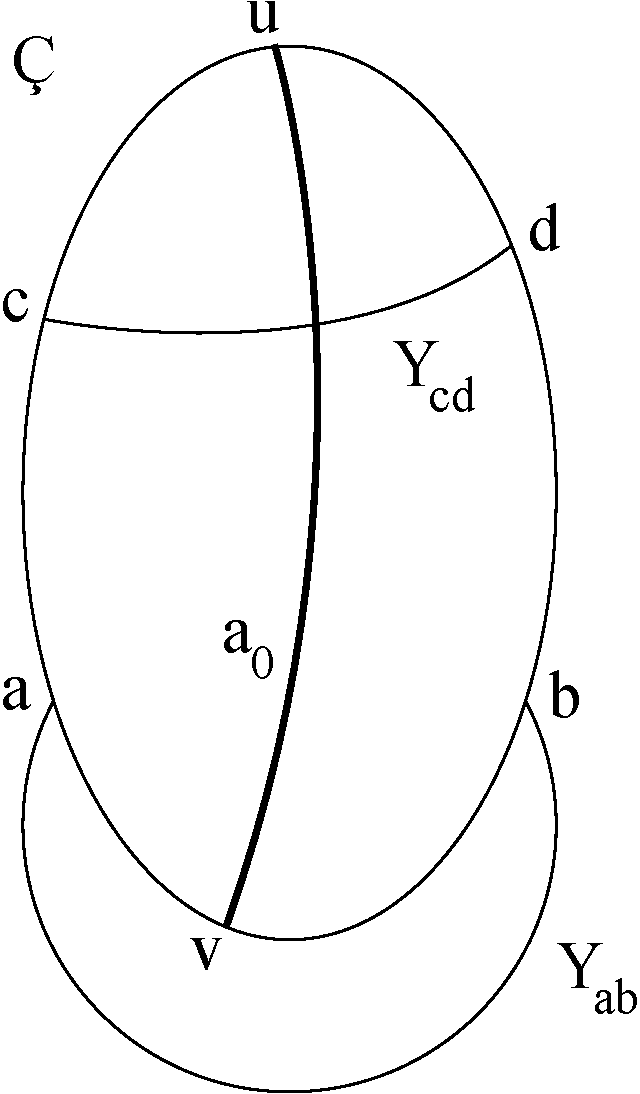
\includegraphics[width=0.20\textwidth]{images/ceyhun-199-fig01}
		\label{fig:durum2ninIncelenmesiA}
	}
  \hspace*{0.2\linewidth}
	\subfigure[]{
		\centering
		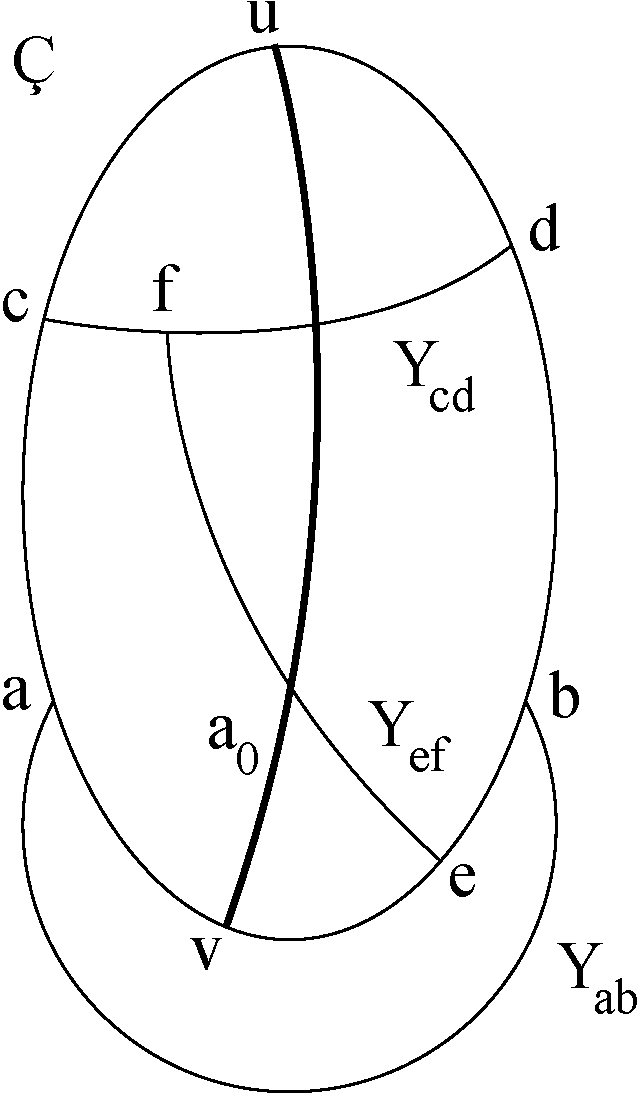
\includegraphics[width=0.20\textwidth]{images/ceyhun-199-fig02}
		\label{fig:durum2ninIncelenmesiB}
	}\\

	\subfigure[]{
		\centering
		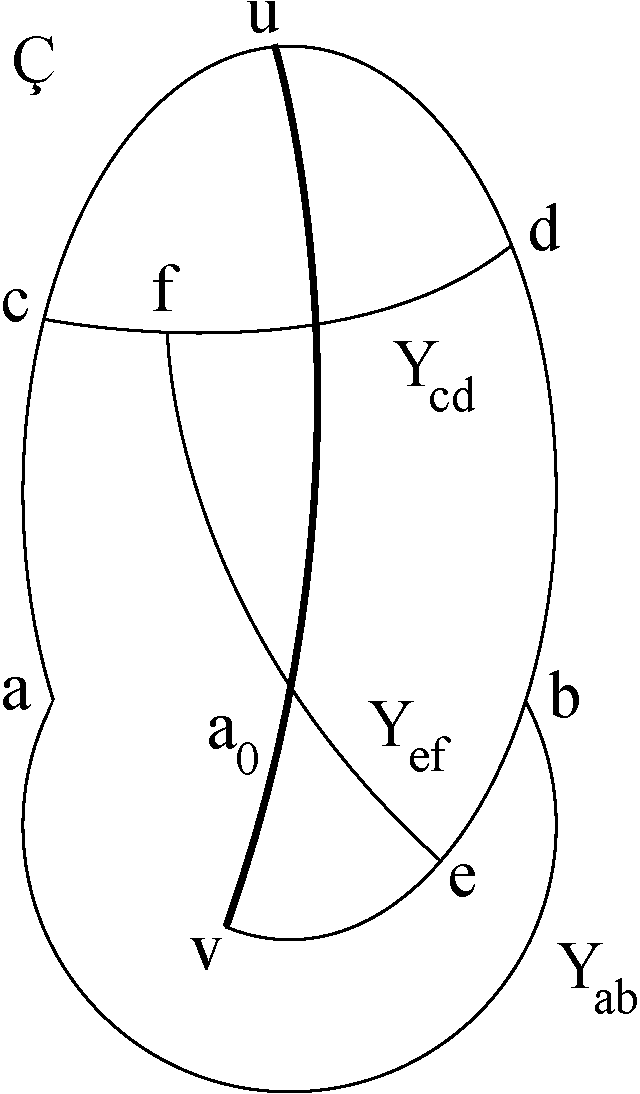
\includegraphics[width=0.20\textwidth]{images/ceyhun-199-fig03}
		\label{fig:durum2ninIncelenmesiC}
	}
  \hspace*{0.2\linewidth}
	\subfigure[]{
		\centering
		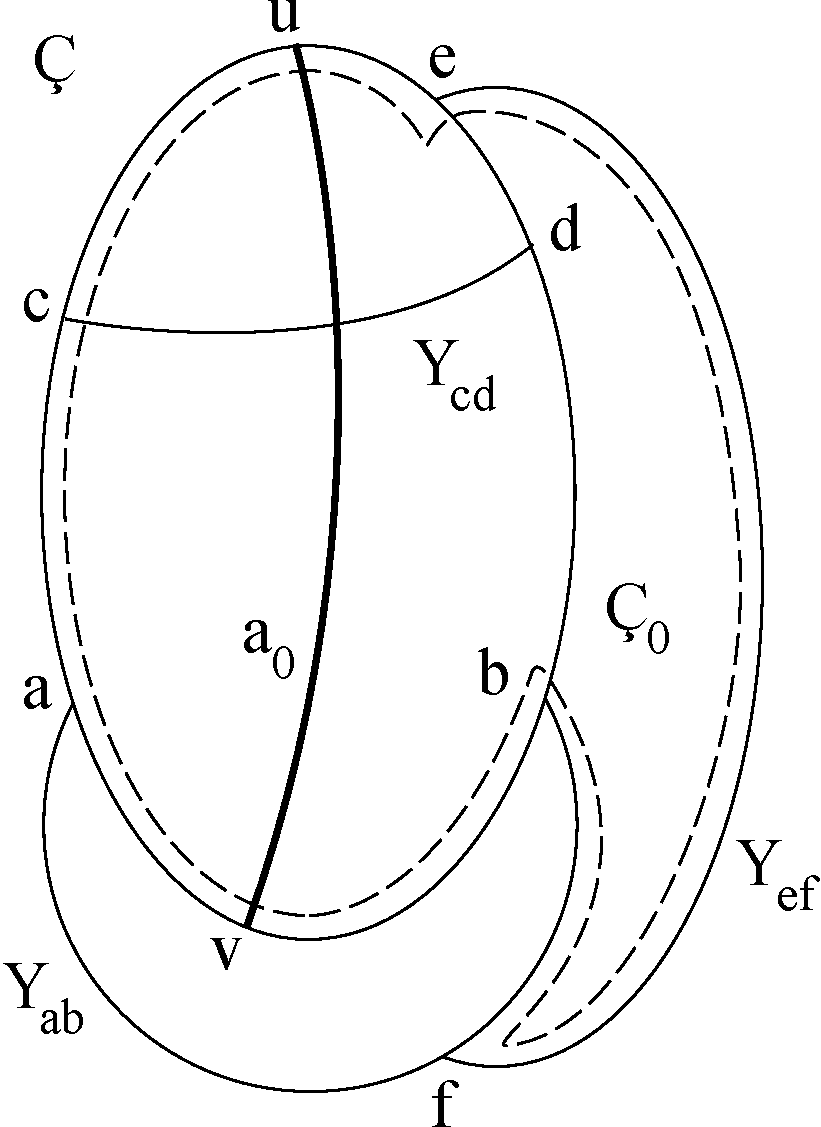
\includegraphics[width=0.25\textwidth]{images/ceyhun-199-fig04}
		\label{fig:durum2ninIncelenmesiD}
	}
	\caption{Durum 2'nin incelenmesi}
\end{figure}

\end{document}
